\section{Experiments and Results}\label{experiments-and-results}
\subsection{Evidence levels and matched exploration protocol}
\label{experimental-setup-and-matched-comparisons}
The primary complete-exploration comparison uses two inspected furniture permutations of one synthetic branching floorplan, with textured assets and partial ideal visible instance/category labels. Each run begins with one actual simulated packet, giving 42.606\% correct-free coverage; the remaining map is unknown. Exact poses, a 0.2\,m circular radius, 120$\times$90 RGB-D at $90^{\circ}$ field of view, 8\,m sensing range and 180 planar scan beams are shared. The measured TSDF uses 6\,cm voxels and 12\,cm truncation. The 256-action cap includes return and is not shortened at first complete coverage, because surface acquisition can continue after floor exploration.

Four new $T=16$ G/S runs are compared with four frozen $T=1$ distribution runs on these same layouts. Temperature was selected only on independent object classification loss. The complete-policy trigger was any changed target in the six fixed prefixes, irrespective of whether its actual branch outcome improved. It was met at one prefix; no new candidate, score coefficient, budget or stopping rule was introduced. Independent evaluation checks the complete action and sensor records, source hashes and native measured meshes. There are no random repeats or independent floorplan replications in this comparison.

Other experiments answer narrower questions. An earlier 24-object split (12 training, six validation, six held-out) selects the conditional-depth scale. A new 48-object set (24 calibration, 24 test) independently evaluates structural temperature and a report-only interval correction. Four viewing conditions per object are dependent observations of that object. Six retained exploration prefixes and 66 previously acquired outbound branches support repeated model diagnostics; reusing them does not increase sample count. The final cue mechanism uses eight separate native outbound branches reused across twelve score conditions. Supplied-graph observation and real-robot pilots have different state and execution assumptions and are retained separately in the supplement.

\subsection{Complete unknown-space coverage and reconstruction}
\label{joint-exploration}
All eight matched entries in Table~\ref{tab:temperature-policy} reach 100\% correctly free reference coverage, return to the initial pose and record zero simulated collisions. At $T=1$, G and S have identical trajectories and native TSDF meshes in each layout. At $T=16$, the left-layout S decision first differs after 54 paid actions, selecting candidate 0 instead of 8 from identical acquired inputs; the actual trajectories first diverge at action 71. The changed policy reaches full coverage at action 97 instead of 88, travels 43.2 instead of 42.0\,m and loses 0.377 percentage points of surface F1. Shelf recall rises by 1.294 points, while cabinet recall falls by 2.834 points. G remains identical to its $T=1$ control. In the right layout, both new policies remain trajectory- and mesh-identical to both $T=1$ controls.

\begin{table}[!htbp]
\centering\small\setlength{\tabcolsep}{4pt}
\caption{Complete unknown-exploration comparisons. All runs start at 42.606\% correct-free coverage, execute 256 actions, finish at 100\%, return and record zero simulated collisions. $A_{100}$ is the first full-coverage action. $T=1$ reuses four previously frozen distribution runs; $T=16$ adds four runs on the same two inspected furniture permutations, not new independent scenes. Surface metrics use measured TSDFs at 5\,cm.}
\label{tab:temperature-policy}
\begin{tabular}{llrrrrrr}
\toprule
Layout & Policy & $T$ & $A_{100}$ & Path (m) & F1 (\%) & Shelf (\%) & Cabinet (\%) \\
\midrule
Left & G & 1 & 88 & 42.0 & 92.758 & 82.170 & 88.709 \\
Left & S & 1 & 88 & 42.0 & 92.758 & 82.170 & 88.709 \\
Left & G & 16 & 88 & 42.0 & 92.758 & 82.170 & 88.709 \\
Left & S & 16 & 97 & 43.2 & 92.381 & 83.464 & 85.874 \\
\midrule
Right & G & 1 & 100 & 43.2 & 92.596 & 81.088 & 79.214 \\
Right & S & 1 & 100 & 43.2 & 92.596 & 81.088 & 79.214 \\
Right & G & 16 & 100 & 43.2 & 92.596 & 81.088 & 79.214 \\
Right & S & 16 & 100 & 43.2 & 92.596 & 81.088 & 79.214 \\
\bottomrule
\end{tabular}
\end{table}

\begin{figure}[!htbp]
\centering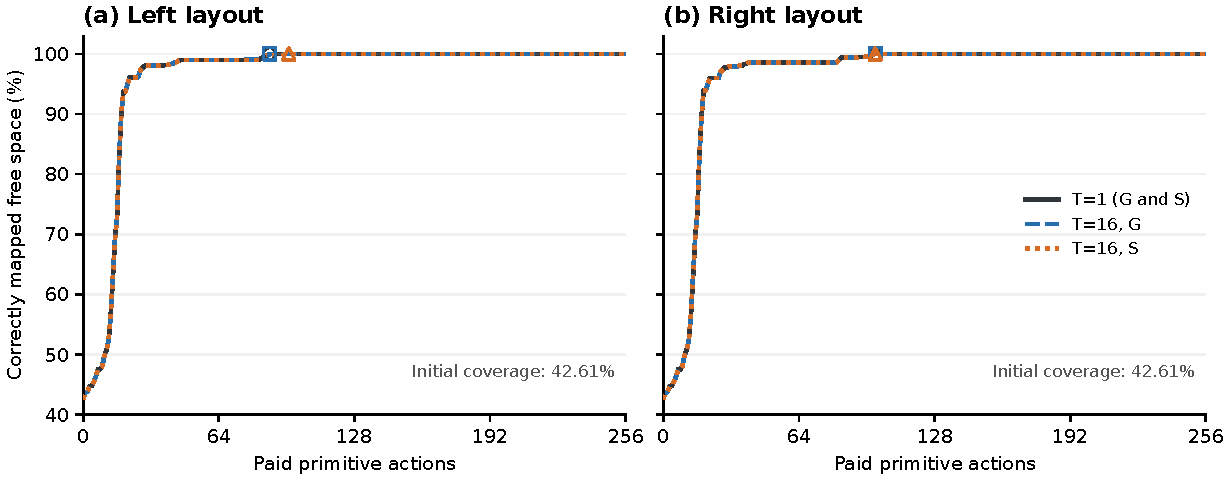
\includegraphics[width=\linewidth]{figures/full_exploration_coverage.pdf}
\caption{Correct-free coverage over all 256 paid actions. The two $T=1$ policies coincide in each layout. Structural temperature produces a left-layout semantic route change that delays complete coverage; all right-layout curves coincide. Curves are related deterministic trajectories on two permutations of one floorplan, not independent scene replicates. The source CSV preserves all eight curves.}
\label{fig:complete-coverage}
\end{figure}

This complete-run result differs from the local branch forecast. At the changed left prefix, the selected S branch adds 0.0434\,m$^2$ more object surface and 1.0581\,m$^2$ more whole-scene surface than the selected G branch, but requires four additional actions and 0.6\,m more travel, with unchanged free coverage. Its favorable surface increment does not compensate for the downstream complete-policy cost and F1 loss. Figure~\ref{fig:complete-coverage} therefore provides a necessary check beyond a changed score or a successful short route.

The earlier matched fixed-extent/distribution/mean comparison helps isolate the effect of representing unresolved extent. In the left layout, distribution and posterior-mean modes improve F1 by 0.377 points, reach full coverage nine actions earlier and travel 1.2\,m less than fixed extent; shelf recall is lower. All right-layout outcomes tie, and posterior mean exactly reproduces the distribution routes. Thus those tests support a layout-specific extent-modeling benefit, without evidence that retaining spread is necessary. Historical coverage-only and joint-without-template controls also remain in the supplement: coverage-only reaches full coverage sooner in the branching layouts, and outperforms G/S coverage and F1 in the earlier three four-room layouts. Completion reward has not established a consistent efficiency advantage over prioritizing unknown coverage.

\subsection{Does predicted visibility become reconstructed surface?}
An acquired-mesh audit finds that 7.67\%/7.48\% of G/S expected template reward already lies within 5\,cm of the current native TSDF, averaging prefixes equally. Suppressing only this duplicate reward reduces development-branch mean absolute error, but four complete matched runs remain trajectory- and mesh-identical to their controls. On twelve separately fixed known-geometry objects, the additive mask instead increases gross-area MAE from 0.1563 to 0.1669\,m$^2$. Duplicate removal alone is therefore not a validated improvement in acquisition prediction or exploration.

The forward estimator in Eq.~\ref{eq:acquisition-reward} is then frozen and evaluated on twelve new known-geometry objects, each with revisit, side and around routes. Against the same fine-basis visibility control, MAE decreases from 0.1532 to 0.0143\,m$^2$; one of the 36 dependent route errors increases. Exact hypothetical geometry makes forecast and actual native meshes identical in this probe, so the remaining error reflects the independent surface quadratures. This isolates the acquisition/fusion operator, not inferred-shape accuracy. On all eleven original candidates at the retained action-54 prefix, fitted forecasts improve ranking relative to the matched mean/fine visibility control but slightly worsen absolute error (Table~\ref{tab:acquisition-alignment}). Both select candidate 8 for G and S; the original distribution's S choice is already changed by the mean/basis approximation. No complete exploration run uses this estimator, and no efficiency gain is inferred from the known-geometry result.
\begin{table}[!htbp]
\centering\small
\caption{Prediction versus actual object gross-new area at 5\,cm. Known-geometry rows average three dependent routes on each of twelve new objects; their single error has no G/S prior. Fitted rows use all eleven original candidates at one retained prefix. The last three share conditional-mean shapes and a 0.06\,m quadrature; the original distribution also differs in geometric integration and basis. MAE is in m$^2$; $\rho$ is candidate Spearman correlation. No complete policy uses the acquisition forecast.}
\label{tab:acquisition-alignment}
\begin{tabular}{llrrrr}
\toprule
Geometry & Estimator & MAE (G) & MAE (S) & $\rho_G$ & $\rho_S$ \\
\midrule
Known geometry & Visibility & 0.1532 & -- & -- & -- \\
Known geometry & Acquisition forecast & 0.0143 & -- & -- & -- \\
Fitted geometry & Original distribution & 0.2061 & 0.1961 & 0.927 & 0.891 \\
Fitted geometry & Mean + fine visibility & 0.3107 & 0.3961 & 0.691 & 0.791 \\
Fitted geometry & Mean + native visibility & 0.3070 & 0.3563 & 0.700 & 0.764 \\
Fitted geometry & Mean + acquisition forecast & 0.3172 & 0.3973 & 0.836 & 0.855 \\
\bottomrule
\end{tabular}
\end{table}



\subsection{Independent structural calibration and its limits}
The structural study fixes 24 new calibration and 24 new test objects before observing predictions, using the same IID mixture of closed/open objects and predeclared geometry mismatch. Each object is measured from front, front--side, around-object and occluded conditions. Generated first-hit depth and visible labels are passed to the actor; hidden dimensions and source meshes are reserved for generation and evaluation. The inferred-axis projection of true geometry defines the depth target, so axis errors are not mislabeled as successful depth estimation. All eight multiple-track fallbacks remain in the test denominator.

Neutral class NLL selects $T=16$ on the calibration objects. On the held-out test objects, neutral NLL falls from 5.0804 to 0.6791, Brier score from 0.3251 to 0.2363, and wrong predictions above 0.9 confidence from 27 to 3. Neutral accuracy remains 63.02\%, consistent with preserving its class ordering. With a supplied correct 9:1 cue, S$^*$ reaches NLL 0.1393 and 96.875\% class accuracy; this is a controlled-prior condition, not an automatic-recognition result. Around-object neutral NLL worsens from 0.0829 to 0.3414, and neutral depth median error increases. The complete condition table and calibration/test rows are retained in the supplement.

These results identify excessive structural confidence as one cause of suppressed category influence, but not the only cause of G/S ties. In the preceding distribution runs, G/S scores differ at seven of 30 left and six of 26 right planning calls while their selected candidates remain identical. Eq.~\ref{eq:semantic-transfer} explains why probability and score changes need not cross the route-ranking margin. The temperature revision makes a category-dependent choice executable, but Table~\ref{tab:temperature-policy} shows no coverage-efficiency benefit.

Conditional extent probability also has important limits. The earlier depth scale was chosen from eight values by training CRPS; 0.01\,m is the grid's lower endpoint, not a demonstrated globally optimal scale. Informative-view CRPS improves in its independent validation/held-out objects, while nominal 95\% intervals under-cover. A separate standard object-level split-conformal diagnostic on the new 24/24 objects raises test case coverage from 61/96 to 93/96 and simultaneous four-condition object coverage from 5/24 to 21/24. Mean interval width increases from 0.278 to 2.316\,m and interval score worsens from 2.140 to 2.704. Its observed object coverage is 87.5\%, not an empirical 95\% success claim. This correction applies only to the unreweighted $T=1$ neutral distribution, leaves all probability masses unchanged and is not used for planning.

\subsection{Controlled category effects on native observation branches}
In two procedural object arrangements, correct, neutral and swapped category cues are evaluated at $T=1$ and $T=16$ using the original candidate generator. Within each arrangement all cues share exactly the same acquired input, particle bank, common score and four candidates. The four available candidates all lie to the right; the experiment therefore tests their actual ranking, not a designed symmetric left/right choice. Across arrangements, rendered depth differs by at most $5\times10^{-7}$\,m, so they are not exact sensor counterfactuals. Eight native outbound routes are executed once and their outcomes reused for the twelve score conditions; all eight reach their endpoints over 114 actions without simulated collision.

At $T=16$ in the right arrangement, the correct cue changes the original target and increases object net-new surface by 1.3565\,m$^2$, improves correctly free coverage gain by 3.328 percentage points and uses two fewer actions. Whole-scene net-new surface simultaneously decreases by 24.1218\,m$^2$. The left arrangement ties at $T=16$; at $T=1$, its correct cue reduces object surface gain while increasing whole-scene gain. These complete contrasts demonstrate that category input can influence native observation allocation, with substantial objective tradeoffs. They do not demonstrate a complete-exploration or uniformly positive semantic effect.

\subsection{Supporting controlled and physical evidence}
A reduced supplied-graph study uses public facility templates, a shared 18-action prefix and a 42-action reference budget. It reports two improvements and two ties in four reference pairs, and a 6.16\% mean joint coverage--surface gain at unchanged planar coverage. Changed-background tests include one improvement and three ties; an independent correction factorial finds a 2.66\% gain from measured correction and no trajectory effect from forecast diagnosis. Planning failures and a larger-budget reversal remain included. These are conditional observation-allocation mechanisms, not unknown-space initialization or stopping rules. Their full formulation, recursion and results are archived in the supplement.

The real-robot record includes completed short joint-exploration episodes, failed returns, control interruptions and map drift. A fresh-map ordered C/S pilot has different initial observations and a failed S return, preventing a matched efficiency ranking. Internal scan unions and quality proxies lack independent geometric ground truth. The physical implementation therefore provides integration evidence; it does not validate the simulated semantic comparison, SLAM accuracy or the complete temperature policy. Hardware experiments are paused following platform damage.
